\chapter{Image Recognition Review}\label{ch:litreview}
  Image recognition tools have undergone a revolution in the past decade.
  Within a significant sector of the research community, previous 
  state of the art models have been all but abandoned in place of newer
  deep learning methods. While there are too many to explore in detail, we give 
  a brief history of some of the relevant methods in this
  chapter, outlining the benefits and drawbacks of each. 

% Include some notation
\section{Notation}
We define standard notation to help the reader better understand figures and
equations. Many of the terms we define here relate to concepts that have not been
introduced yet, so may be unclear until later.

\begin{itemize}
  \item \textbf{Pixel coordinates}\\
    When referencing spatial coordinates in an image, the preferred index
    is $\bmu{u}$ for a 2D vector of coordinates, or $[u_1,u_2]$ if we wish to
    specify the coordinates explicitly. $u_1$ indexes rows from top to bottom
    of an image, and $u_2$ indexes columns from left to right. We typically use
    $H\x W$ for the size of the image, (but this is less strict). I.e.,\ 
    $u_1 \in \{0, 1, \ldots H-1\}$ and $u_2 \in {0, 1, \ldots W-1}$. 

  \item \textbf{Convolutional networks}\\
    Image convolutional neural networks often work with 4-dimensional arrays. In particular,
    mini-batches of images with multiple channels. When we need to, we index over the 
    minibatch with the variable $n$ and over the channel dimension with $c$. For example, we can
    index an activation $\bmu{x}$ by $\bmu{x}[n, c, u_1, u_2]$.

    To distinguish between features, filters, weights and biases of different
    levels in a deep network, we may add a layer subscript, or $l$ for the
    general case, i.e.,\ $\bmu{z}_l[n, c, \bmu{u}]$ indexes the feature map at the $l$-th
    layer of a deep network. 
    
  \item \textbf{Fourier transforms}\\
    When referring to the Fourier transform of a function, $f$, we typically
    adopt the overbar notation: i.e., $\mathcal{F}\{f\} = \bar{f}$. 

  \item \textbf{Wavelet Filter Banks}\\
    Using standard notation, we define the scaling function as $\phi$ and the wavelet function 
    as $\psi$. For a filter bank implementation of a wavelet transform, we use $h$ for analysis and
    $g$ for synthesis filters.    

    In a multiscale environment, $j$ indexes scale from $\{1,2, \ldots, J\}$. For 2D complex
    wavelets, $\theta$ indexes the orientation at which the wavelet has the largest response, i.e.,\
    $\psi_{\theta, j}$ refers to the wavelet at orientation $\theta$ at the $j$-th scale.

\end{itemize}


\section{Datasets}\label{sec:datasets}
  When considering an image recognition model, it is essential to have a set of
  images to build your model on, and to compare performance to other models.
  This naturally involves a choice at the outset of your design.  Whatever
  choice is made, it is important to know the benefits of your dataset, its
  limitations, and most importantly, to remember that your model should still
  be valid outside of it.

  In current image recognition and classification there are a handful of
  datasets which are used in the vast majority of literature. In particular,
  the two most commonly used are ImageNet \citep{russakovsky_imagenet_2015}
  (part of the ongoing challenge --- ImageNet Large Scale Visual Recognition
  Competition) and \cifar\citep{krizhevsky_learning_2009}. These are at two
  ends of our decision spectrum. 
  
  ImageNet is a very large dataset, consisting of 1000 classes with a total of
  1.4 million images. Each image is typically a few hundred pixels wide and
  tall, but this does vary image to image. Beyond the size of the dataset and
  the size of the images, it is also useful for having:
  
  \begin{itemize}
    \item Objects at varying scales from being only a few pixels in the image,
      to taking up the entire image.
    \item Objects with a varying number of instances in the images. I.e.,\ it
      does not limit an object to only appear once in an image.
    \item Varying degrees of clutter in the images.
    \item Varying amounts of texture on the objects of interest.
  \end{itemize}
  Some examples are shown in \autoref{fig:imagenet}

  \begin{figure}
    \centering
      % \makebox[\textwidth]{\includegraphics[width=1\textwidth]{images/imagenet_1000.jpg}}
      \caption[Sample images from ImageNet]
      {Sample images from ImageNet. These images have been cropped to
      make them square; the raw images vary in size and aspect ratio, but are
      all at least a few hundred pixels wide and tall.}
      \label{fig:imagenet}
  \end{figure}

  On the other hand, \cifar\ is a dataset containing only $60000$ images from
  10 different classes. The images are tiny, all $32\x 32$ pixels\footnote{%
  The source images for \cifar\ were not necessarily square, but all have
  been scaled to be \emph{before} including them in the dataset.}.
  The key benefit of this dataset is its size. Both the images and the training
  set are small, which means training time is considerably reduced. This can
  allow us to test many different models and get feedback quickly. Some
  examples of these images are shown in \autoref{fig:cifar10}. Such small images are
  appealing to train models on, but when we as humans struggle to see the
  detail in them, perhaps too much information has been thrown away. On top of
  this criticism, most of the objects of interest are centred on the image,
  with little background clutter.

  \begin{figure} 
    \centering
      % \makebox[\textwidth][c]{\includegraphics[width=1.1\textwidth]{images/cifar10.png}}
      \caption[Sample images from \cifar] 
      {Sample images from the 10 classes of \cifar.}
      \label{fig:cifar10} 
  \end{figure}

  There are a few other datasets that also deserve a mention:
  \begin{itemize}
    \item Pascal-VOC: The state of the art dataset before ImageNet, contains
      $21738$ images in 20 classes. Like ImageNet, the images are typically
      medium resolution (a few hundred pixels in each direction).
    \item Caltech-101 and Caltech-256: Similar image size to ImageNet, but many
      fewer samples per class (15--30). Caltech is still often used if the
      goal of the model is training on small amounts of data.
    \item Microsoft COCO (Common Objects in Context)
      \citep{lin_microsoft_2014}: MS COCO
      has fewer object categories than ImageNet, and about one quarter of the
      number of images, but its $328000$ images are fully segmented.
      It is the state of the art dataset currently being used for object
      detection and localization challenges.
  \end{itemize}

\section{Sparse Dictionary Learning}
  The work by \citeauthor{olshausen_emergence_1996}
  in~\citep{olshausen_emergence_1996, olshausen_sparse_1997} show that a system
  will learn the Gabor-like filters associated with the mammalian V1 cortex, if
  the constraints of sparsity and minimizing reconstruction error are used.

  Introducing sparsity as a constraint may not seem obvious at first. The
  authors suggest though that it should follow from the intuition that natural
  images may be described in terms of a small number of structural primitives
  (e.g.\ edges, lines)\cite{field_what_1994}, which is also supported by the
  high kurtosis (fourth order statistic) seen in natural
  images\citep{field_scale-invariance_1993}.

  The problem is defined as trying to find $\phi_{i}$\footnote{The use of
  $\phi$ is deliberate here, to keep it in line with the tradition of it
  representing an \emph{analysis} function in the wavelet community} that
  create a dictionary, so that the effective dimensionality of any image can be
  reduced:
  % Equation representing the reconstruction of an image
  $$\hat{I}(u_1, u_2) = \sum_{i} a_{i} \phi_{i} $$

  PCA is a natural starting point to choose to solve this problem, as it
  attempts to find a set of mutually orthogonal basis functions that capture the
  directions of maximum variances of the data, and so can maximally reduce the
  dimensionality for a given reconstruction error, or alternatively, requires
  the fewest dictionary elements to best represent the data (due to the
  orthogonality constraint of PCA). The resulting learned dictionary is shown
  in \autoref{fig:olshausen_pca}. Unfortunately, the shortcomings of this
  approach are clear. These filters are not at all localized, and further, do
  not resemble any known cortical receptive fields.

  % Figure of the PCA images from Olshausen's letter to nature
  \begin{figure}
    \begin{center}
      % \includegraphics[width=0.6\textwidth]{images/olshausen_pca.png}
      \caption[Principal components learned on natural images]
              {Principal components calculated on $8\times 8$ image patches from
               natural images, ordered in increasing variance. Taken from
               \citep{olshausen_emergence_1996}.}
       \label{fig:olshausen_pca}
    \end{center}
  \end{figure}

  \citeauthor{olshausen_emergence_1996} instead define a cost function that
  promotes sparsity as well as the reconstruction error, given by:
  %\begin{center}
    \begin{eqnarray}
    E & = & -\left[\text{preserve information}\right]
            -\lambda \left[\text{sparseness of $a_{i}$}\right] \\
      & = & \sum_{u_1,u_2} {\left[I(u_1,u_2)-\sum_{i} a_{i} \phi_{i} \right]}^2 + 
            \lambda \sum_{i} S \frac{a_{i}}{\sigma}
    \end{eqnarray}
  %\end{center}

  where $\sigma$ is a scaling constant, and $S(x)$ is a function that promotes
  sparsity, such as $\exp{-x^2}$, $\log (1+x^2)$, or $|x|$. Finding $a_i$ and
  $\phi_i$ is then done per image patch by holding one constant, and using it to
  find/update the other. The resulting basis functions are shown in
  \autoref{fig:olshausen_sparse}.

  % Figure of the sparse representations learned
  \begin{figure}
    \begin{center}
      % \includegraphics[width=\textwidth]{images/olshausen_sparse.png}
      \caption[Olshausen and Field sparse dictionary basis functions]
      {Sparse dictionary basis functions found from training on $16\times 16$ patches of
               natural images. Taken from \citep{olshausen_emergence_1996}.}
       \label{fig:olshausen_sparse}
    \end{center}
  \end{figure}

  The basis functions learned by this method both resemble the activations found
  in the V1 cortex, as well as those developed independently by engineers to
  efficiently code images. This suggests that the V1 cortex may be attempting to
  compress input into statistically independent and sparse representations.

\section{SIFT Detectors}
  SIFT, or Scale Invariant Feature Transforms, were first introduced by
  \citet{lowe_object_1999} and described in depth in \citep{lowe_distinctive_2004}.
  They are currently used extensively for image matching problems. They create
  a set of features in an image that are designed to be invariant to image scale and rotation,
  as well as illumination changes. 

  The algorithm has two main steps to it:
  \begin{enumerate}
  \item Keypoint detection by finding scale-space extrema --- `blobs' with
    Laplacian of Gaussian (LoG) filters 
  \item Generate feature vectors for each keypoint
  \end{enumerate}
  `Scale' in the first step refers to the width of LoG filters (their $\sigma$
  parameter). They use four scales per octave, so the image is filtered
  successively by a LoG which has $\sigma_{i+1} = 2^{\frac{1}{3}}\sigma_i$. The
  increasing width of the LoG means we are successively searching coarser and
  coarser scales. Maxima are then found by comparing outputs to its neighbours in
  scale and space, and choosing the max. This point is then checked to see if it
  has sufficient curvature and rejected if not. If this value is above a set threshold,
  then that coordinate in scale and space $(x,y, \sigma_i^2)$ is marked as
  a keypoint, and given to the feature generator.

  To account for rotations across images, once a keypoint is found, its dominant
  orientation is first determined before generating any features. This is done by
  calculating the direction with the greatest gradient with a resolution of $10\degs$. 
  Further processing is done relative to this orientation. If there
  were multiple large orientations (this happens roughly $15\%$ of the time),
  then multiple feature vectors are created.

  Once this has been done, a feature is generated by finding gradients in a patch
  of pixels around the keypoint in the same scale. These gradients are then put
  into much coarser bins (usually around $45\degs$), in sub-patches around the
  keypoint. These are then unravelled to make a low-dimensional vector to
  represent that keypoint. This is shown more clearly in
  \autoref{fig:sift_gradients}.

  \begin{figure}
    \begin{center}
      % \includegraphics[scale=0.5]{images/sift_gradients.png}
      \caption[SIFT descriptor applied to a keypoint]
              {Keypoint descriptor for a $8 \x 8$ patch of pixels
               \citep{lowe_distinctive_2004}. The left shows gradients being calculated per
               pixel, then weighted by a smooth gaussian filter. The right shows these
               gradients put into bins of 8 orientations, and then combined in
               4 smaller $4 \x 4$ pixel areas. Unravelling this would give a 
               $4 \x 8 = 32$ long feature vector}
       \label{fig:sift_gradients}
    \end{center}
  \end{figure}

%\section{HOG}
%\section{Neural Networks}
% 
  % The nature paper cites papers 31-34
  % The researchers introduced
  % unsupervised learning procedures that could create layers of
  % feature detectors without requiring labelled data. The objective in
  % learning each layer of feature detectors was to be able to reconstruct
  % or model the activities of feature detectors (or raw inputs) in the layer
  % below. By ‘pre-training’ several layers of progressively more complex
  % feature detectors using this reconstruction objective, the weights of a
  % deep network could be initialized to sensible values. A final layer of
  % output units could then be added to the top of the network and the
  % whole deep system could be fine-tuned using standard backpropagation33–
  % 35.
% 
\section{Convolutional Neural Networks}\label{sec:cnns}
  Convolutional Neural Networks (CNNs) were initially introduced by \citet{lecun_backpropagation_1989} in
  \citep{lecun_backpropagation_1989}. Due to the difficulty of training and
  initializing them, they failed to be popular for more than two decades.  This
  changed in 2012, when advancements in pre-training with unsupervised networks
  \citep{bengio_greedy_2007}, the use of an improved non-linearity --- the Rectified Linear
  Unit, or ReLU, new regularization methods\citep{hinton_improving_2012}, and
  access to more powerful computers in graphics cards, or GPUs, allowed
  Krizhevsky, Sutskever and Hinton  to develop
  AlexNet\citep{krizhevsky_imagenet_2012}. This network nearly halved the
  previous state of the art's error rate.  Since then, interest in them has
  expanded very rapidly, and they have been successfully applied to object
  detection~\citep{ren_object_2015} and human pose estimation
  \citep{tompson_efficient_2015}. It would take a considerable amount of effort
  to document the details of all the current enhancements and tricks many
  researches are using to squeeze extra accuracy, so for the purposes of this
  report we restrict ourselves to their generic design, with some time spent
  describing some of the more promising enhancements. 
  
  We would like to make note of some of the key architectures
  in the history of CNNs, which we, unfortunately, do not have space to describe:
  \begin{itemize}
    \item Yann LeCun's LeNet-5~\citep{lecun_gradient-based_1998}, the state of the art
      design for postal digit recognition on the MNIST dataset.
    \item Google's GoogLeNet~\citep{szegedy_going_2015} achieved $6.67\%$ top-5
      error on ILSVRC2014, introducing the new `inception' architecture, which
      uses combinations of $1\x 1$, $3\x 3$ and $5\x 5$ convolutions.
    \item Oxford's VGG~\citep{simonyan_very_2014} --- $6.8\%$ and runner up in
      ILSVRC2014. The VGG design is very similar to AlexNet but was roughly
      twice as deep. More convolutional layers were used, but with smaller
      support --- only $3\x 3$. These were often stacked directly on top of
      each other without a non-linearity in between, to give the effective
      support of a $5\x 5$ filter.
    \item Microsoft Research's ResNet~\citep{he_deep_2015} achieved $4.5\%$ top-5 
      error and was the winner of ILSVRC2015. This network we will talk briefly
      about, as it introduced a very nice novel layer --- the residual layer.
  \end{itemize}

  Despite the many variations of CNN architectures currently being used, most
  follow roughly the same recipe (shown in \autoref{fig:cnn_generic}):
  \begin{figure}
    \centering
      % 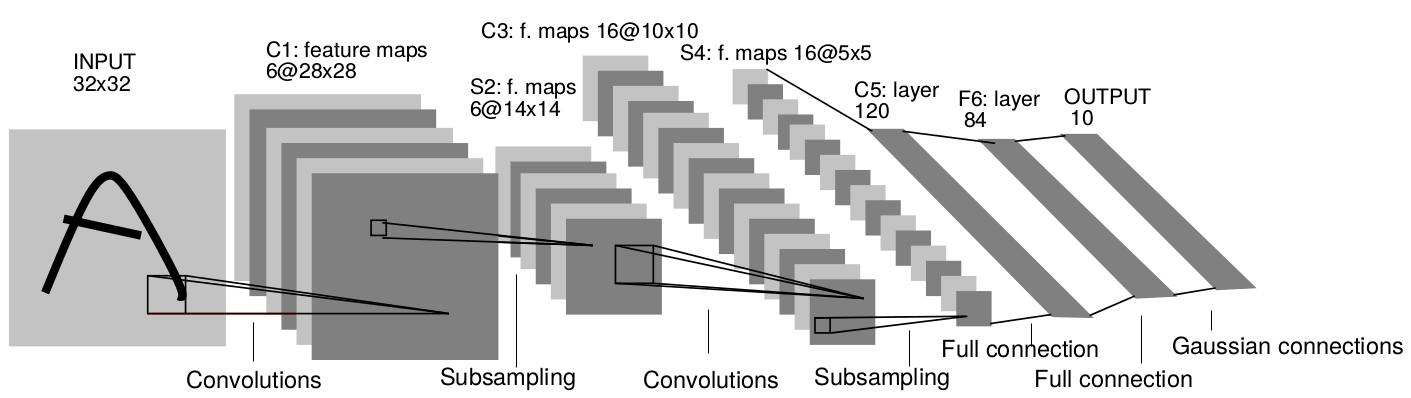
\includegraphics[width=\textwidth]{images/cnns.png}
      \caption[Standard CNN architecture]
              {Standard CNN architecture. Taken
              from~\citep{lecun_gradient-based_1998}}\label{fig:cnn_generic}
  \end{figure}

\subsection{Input Layer}\label{sec:cnn_input} 
  The input is typically scaled, often removing the mean and dividing by the
  variance. This helps initialize the network in such a way as to operate
  within the region of activation of the non-linearities, which are necessary
  to turn linear convolutions into non-linear functions. 

\subsection{Convolutional Layers}\label{sec:cnn_conv} 
  The image/layer of features is convolved by a set of filters.
  The filters are typically small, ranging from $3\x 3$ in ResNet and VGG
  to $11\x 11$ in AlexNet. We have quoted only spatial size
  here, as the filters in a CNN are always \emph{fully connected in depth} ---
  i.e.,\ they will match the number of channels their input has.

  For an input $\bmu{x} \in \mathbb{R}^{H\x W\x D}$, and filters 
  $\bmu{f} \in \mathbb{R}^{H'\x W'  \x D \x D''}$ ($D''$ is the 
  number of filters), our output $\bmu{z} \in
  \mathbb{R}^{H''\x W'' \x D''}$ will be given by:
  \begin{equation}
    z[u_1, u_2, d''] = b[d''] + \sum_{i=-\frac{H'}{2}}^{\frac{H'}{2}-1}
                       \sum_{j=-\frac{W'}{2}}^{\frac{W'}{2}-1}  \sum_{k=0}^{D-1}  
                        f[i, j, k, d''] x[u_1-i, u_2-j, k]
  \end{equation}

  The stride is another important feature to note about the convolutional
  layer. Historically, unit stride was used \citep{lecun_gradient-based_1998,
  krizhevsky_imagenet_2012}, but newer models started to use stride 2 
   \citep{szegedy_going_2015}. Since then, designers vacillate between whether
   to keep unit stride or not, with some newer designs using both
   \citep{szegedy_inception-v4_2016}.

\subsection{Pooling Layers}\label{sec:cnn_pooling} 
  Typically following a convolutional layer (but not strictly), activations are subsampled with
  max pooling. Pooling adds some invariance to shifts smaller than the pooling
  size at the cost of information loss. For this reason, small pooling is
  typically done often $2\x 2$ or $3\x 3$, and the invariance to larger shifts
  comes after multiple pooling (and convolutional) layers.
  
  While initial designs of max pooling would do it in non-overlapping regions, 
  AlexNet used $3\x 3$ pooling with stride 2 in their breakthrough design,
  quoting that it gave them an increase in accuracy of roughly $0.5\%$ and
  helped prevent their network from `overfitting'. More recent networks will
  typically employ either this or the original $2\x 2$ pooling with stride 2,
  see \autoref{fig:maxpool}. A review of pooling methods in
  \citep{mishkin_systematic_2016} found them both to perform equally well.
  
  \begin{figure}
    \centering
    % \subfloat[]{%
        % \input{tikz/maxpool.tex}\label{fig:maxpool_tight}
    % }
%    \newline
    \centering
    % \subfloat[]{%
        % \input{tikz/maxpool_overlap.tex}\label{fig:maxpool_overlap}
    % }
    \caption[Tight vs.\ overlapping pooling]
            {\subref{fig:maxpool_tight} Tight $2\x 2$ pooling with stride 2, vs
            \subref{fig:maxpool_overlap} overlapping $3\x 3$ pooling with
            stride 2. Overlapping pooling has the possibility of having one
            large activation copied to two positions in the reduced size
            feature map, which places more emphasis on the odd columns.}
    \label{fig:maxpool}
  \end{figure}
  
\subsection{Activation Functions}\label{sec:cnn_neurons}
  Activation functions, neurons, or non-linearities, are the core of a neural networks
  expressibility. Historically, they were sigmoid or tanh functions, but these
  have been replaced recently by the Rectified Linear Unit (ReLU), which has
  equation $g(x) = \max(0,x)$. A ReLU
  non-linearity has two main advantages over its smoother predecessors~\citep{%
  glorot_deep_2011, nair_rectified_2010}.
  \begin{enumerate}
  \item It is less sensitive to initial conditions as the gradients that
    backpropagate through it will be large even if $x$ is large. A common
    observation of sigmoid and tanh non-linearities was that their learning would
    be slow for quite some time until the neurons came out of saturation, and then
    their accuracy would increase rapidly before levelling out again at
    a minimum~\citep{glorot_understanding_2010}. The ReLU, on the other hand, has
    constant gradient.
  \item It promotes sparsity in outputs, by setting them to a hard 0. Studies
    on brain energy expenditure suggest that neurons encode information in
    a sparse manner. \citet{lennie_cost_2003} estimates the percentage of
    neurons active at the same time to be between 1 and 4\%. Sigmoid and tanh
    functions will typically have \emph{all} neurons firing, while 
    the ReLU can allow neurons to fully turn off.
  \end{enumerate}

  \begin{figure}
    \centering
      % \section{Wavelet-Based Nonlinearities}\label{sec:ch6:nonlinearities}
Returning to the goals from \autoref{sec:ch6:learning}, the experiments from the
previous section have shown that while it is possible to use a wavelet gain
layer ($G$) in place of a convolutional layer ($H$), this may come with a small
performance penalty. Ignoring this effect for the moment, in this section, we
continue with our investigations into learning in the wavelet domain. In
particular, is it possible to replace a pixel domain nonlinearity $\sigma$ with
a wavelet-based one $\sigma_w$?

But what sensible nonlinearity should be used? Two particular options are good initial
candidates:
\begin{enumerate}
  \item The ReLU: this is a mainstay of most modern neural networks and has
    proved invaluable in the pixel domain. Its pseudo-nonlinearity
    ($\F{ReLU}(Ax) = A\F{ReLU}(x)$) makes learning less dependent on signal
    amplitudes. Perhaps its sparsifying
    properties will work well on wavelet coefficients too. 
  \item Thresholding: a technique commonly applied to wavelet
    coefficients for denoising and compression. Many proponents of compressed
    sensing and dictionary learning even like to compare soft thresholding to a
    two-sided ReLU \cite{papyan_theoretical_2018, papyan_convolutional_2017-1}.
\end{enumerate}

In this section, we will look at both and see if they improve the gain
layer. If they do, it would the be possible to connect multiple layers in the
wavelet domain, avoiding the necessity to do inverse wavelet transforms after
learning.

\subsection{ReLUs in the Wavelet Domain}
Applying the ReLU to the real lowpass coefficients is not difficult, but it does
not generalize so easily to complex coefficients. The simplest option is to apply
it independently to the real and imaginary coefficients, effectively only
selecting one quadrant of the complex plane:
\begin{align}
  u_{lp} &= \F{max}(0,\ v_{lp}) \\
  u_{j} &= \F{max}(0,\ \real{v_{j}}) + j\F{max}(0,\ \imag{v_j}) \label{eq:ch6:relu_bp}
\end{align}

Another option is to apply it to the magnitude of the bandpass coefficients. Of
course, these are all strictly positive so the ReLU on its own would not do
anything. However, they can be arbitrarily scaled and shifted by using a batch
normalization layer. Then the magnitude could shift to (invalid) negative
values, which can then be rectified by the ReLU.

Dropping the scale subscript $j$ for clarity (we need it for the square root of 
negative 1), let a bandpass coefficient at a given scale be
$v = r_v e^{j\theta_v}$ and define
$\mu_r = \mathbb{E}[r_v]$ and $\sigma_r^2 = \mathbb{E}[(r_v-\mu_r)^2]$, then
applying batch-normalization and the ReLU to the magnitude of $v_j$ means we
get:
\begin{align}
  r_u &= \F{ReLU}(BN(r_v)) = \max(0,\ \gamma \frac{r_v-\mu_r}{\sigma_r} + \beta) \label{eq:ch6:magrelu_bp} \\
  u &= r_u e^{j\theta_v} \label{eq:ch6:magrelu_bp2}
\end{align}
This also works equivalently on the lowpass coefficients, although $v_{lp}$ can
be negative unlike $r_v$:
\begin{equation}
  u_{lp} = \F{ReLU}(BN(v_{lp})) = \max(0, \gamma' \frac{v_{lp} - \mu_{lp}}{\sigma_{lp}} + \beta') \label{eq:ch6:bnrelu_lp}
\end{equation}
%
\subsection{Thresholding}
For $t \in \reals$ and $z = re^{j\theta} \in \complexes$ the pointwise hard thresholding is:
\begin{align}
  \mathcal{H}(z, t) &= \left\{ \begin{array}{ll}
    z & r \geq t \\
    0 & r < t\\
  \end{array} \right. \\
  &= \indic(r > t) z
\end{align}
and the pointwise soft thresholding is:
\begin{align}
  \mathcal{S}(z, t) &= \left\{ \begin{array}{ll}
    (r-t)e^{j\theta} & r \geq t \\
    0 & r < t\\
  \end{array} \right. \\
  &= \max(0, r - t)e^{j\theta} \label{eq:ch6:relu_st}
\end{align}
Note that \eqref{eq:ch6:relu_st} is very similar to \eqref{eq:ch6:magrelu_bp} and \eqref{eq:ch6:magrelu_bp2}.
We can rewrite \eqref{eq:ch6:magrelu_bp} by taking the strictly positive terms
$\gamma$, $\sigma$ outside of the $\max$ operator:
\begin{align}
  r_u &= \max(0, \gamma \frac{r_v-\mu_r}{\sigma_r} + \beta) \\
      &= \frac{\gamma}{\sigma_r}\max\left(0, r_v - \left(\mu_r - \frac{\sigma_r\beta}{\gamma}\right)\right) \label{eq:ch6:bnrelu_soft}
\end{align}
then if $t' = \mu_v - \frac{\sigma_r\beta}{\gamma} > 0$, \textbf{doing batch
normalization followed by a ReLU on the magnitude of the complex coefficients is the
same as soft shrinkage with threshold $t'$, scaled by a factor
$\frac{\gamma}{\sigma_r}$}.

The same analogy does not apply to the lowpass
coefficients, as $v_{lp}$ is not strictly positive.

While soft thresholding is similar to batch normalizations and ReLUs, we would also like
to test how well it performs as a sparsity-inducing wavelet nonlinearity.
To do this, we can:
\begin{itemize}
  \item Learn the threshold $t$
  \item Adapt $t$ as a function of the distribution of activations to achieve a desired sparsity level.
\end{itemize}
In early experiments, we found that trying to set
desired sparsity levels by tracking the standard deviation of the statistics
and setting a threshold as a function of it performed very poorly (causing a
drop in top-1 accuracy of at least 10\%).
Instead, we choose to learn a threshold $t$. We make this an unconstrained
optimization problem by changing \eqref{eq:ch6:relu_st} to:
\begin{equation}
  \mathcal{S}(v, t) = \max(0, r-|t|)e^{j\theta}  \label{eq:ch6:relu_st2}
\end{equation}

Learning a threshold is only possible for soft thresholding, as $\dydx{L}{t}$ is
not defined for hard thresholding. Like batch normalization, we learn
independent thresholds $t$ for each channel.

      \caption[Differences in non-linearities]
              {Differences in non-linearities. Green --- the \emph{sigmoid} function, 
               Blue --- the \emph{tanh} function, and Red --- the \emph{ReLU}\@. The ReLU
               solves the problem of small gradients outside of the activation
               region (around $x=0$) as well as promoting sparsity.}\label{fig:nonlinearities}
  \end{figure}

\subsection{Fully Connected Layers}\label{sec:cnn_fullyconnected}
  The convolutuion, pooling, and activation layers all
  conceptually form part of the \emph{feature extraction} stage of a CNN\@. One
  or more fully connected layers are usually placed after these layers to form
  the \emph{classifier}. One of the most elegant and indeed most powerful
  features of CNNs is this seamless connection between the \emph{feature
  extraction} and \emph{classifier} sub-networks, allowing the backpropagation
  of gradients through all layers of the entire network.

  The fully connected layers in a CNN are the same as those in a classical
  Neural Network (NN), in that they compute a dot product between their input
  vector and a weight vector:
  \begin{equation}
    z_i = \sum_{j} W_{ij}x_j
  \end{equation}
  The final output of the Fully Connected layer typically has the same number
  of outputs as the number of classes $C$ in the classification problem.

\subsection{Loss Function}
  For a given sample $q=(x, y)$, the loss
  function is used to measure the cost of predicting $\hat{y}$ when the
  true label was $y$. We define a loss function $\loss (y, \hat{y})$. 
  A CNN is a deterministic
  function of its weights and inputs, $f(x,w)$ so this can be written as $\loss
  (y, f(x,w))$, or simply $\loss(y, x, w)$.
  
  It is important to remember that we can choose
  to penalize errors however we please, although for CNNs, the vast majority of
  networks use the same loss function --- the softmax loss. Some networks have
  experimented with using the hinge loss function (or `SVM loss'), stating they
  could achieve improved results \citep{gu_recent_2015,tang_deep_2013}. 
  \begin{enumerate}

  \item \emph{Softmax Loss:} The more common of the two, the softmax turns
    predictions into non-negative, unit summing values, giving the sense of
    outputting a probability distribution. The softmax function is applied to
    the $C$ outputs of the network (one for each class):
    \begin{equation}
      p_j = \frac{e^{(f(x, w))(j)}}{\sum\limits_{k=1}^{C}e^{(f(x,w))(k)}}
    \end{equation}
    where we have indexed the $c$-th element of the output vector $f(x,w)$ with
      $(f(x,w))(c)$. The softmax \emph{loss} is then defined as:
    \begin{equation}
      \loss (y_i, x, w)
      = \sum_{j=1}^{C} \mathbbm{1}\{y_i=j\} \log p_j
    \end{equation}
    Where $\mathbbm{1}$ is the indicator function, and $y_i$ is the true label
    for input $i$.

  \item \emph{Hinge Loss:} The same loss function from Support Vector
    Machines (SVMs) can be used to train a large margin classifier in a CNN:\@
    \begin{equation}
      \loss(y,x,w) = \sum_{l=1}^{C} 
        {\left[ \max(0, 1 - \delta(y_i,l) w^{T}x_{i}) \right]}^p \label{eq:nn_hinge_loss}
    \end{equation}
    Using a hinge loss like this introduces extra parameters, which would
    typically replace the final fully connected layer. The $p$ parameter in
    \autoref{eq:nn_hinge_loss} can be used to choose $\ell^1$ Hinge-Loss, or
    $\ell^2$ Squared Hinge-Loss. 

  \end{enumerate}
  

\subsubsection{Regularization}
  Weight regularization, such as an $\ell^2$ penalty is often given to the
  learned parameters of a system. This applies to the parameters of the fully
  connected, as well as the convolutional layers in a CNN\@. These are added to
  the loss function. Often the two loss components are differentiated between by
  their monikers - `data loss' and `regularization loss'. The above 
  equation then becomes:
  \begin{equation}
    \mathcal{L} = \mathcal{L}_{data} + \underbrace{\frac{1}{2}\lambda_{fc}
    \sum_{i=1}^{L_{fc}} \sum_{j} \sum_{k} {(w_{i}[j,k])}^2}_{\text{fully connected
    loss}} +
    \underbrace{\frac{1}{2}\lambda_{c} \sum_{i=1}^{L_c} \sum_{u_1} \sum_{u_2} \sum_{d}
    \sum_{n} \left(f_i[u_1,u_2,d,n]\right)^2}_{\text{convolutional loss}}
  \end{equation}

  Where $\lambda_{fc}$ and $\lambda_{c}$ control the regularization parameters
  for the network. These are often also called `weight decay' parameters.

  The choice to split the $\lambda$'s between fully connected and convolutional
  layers was relatively arbitrary. More advanced networks can make $\lambda$
  a function of the layer. 

\subsubsection{Empirical Risk vs Expected Risk}
  So far we have defined the loss function for a given data point $(x^{(i)},
  y^{(i)})$. Typically, we want our network to be able to generalize to the
  true real world joint distribution $P(x,y)$, minimizing the expected risk ($R_E$) of
  loss:
  \begin{equation}
    R_E(f(x,w)) = \int \loss(y,f(x,w)) dP(x,y)
  \end{equation}
  Instead, we are limited to the training set, so we must settle for the
  empirical risk ($R_{EMP}$):
  \begin{equation}
    R_{EMP}(f(x,w)) = \frac{1}{N} \sum_{i=1}^{N} \loss( y^{(i)},f(x^{(i)}, w))
    \label{eq:empirical_risk}
  \end{equation}

\subsection{Gradient descent vs Stochastic Gradient Descent vs Mini-Batches}
  We can minimize \autoref{eq:empirical_risk} with \emph{gradient descent}
  \citep{rumelhart_parallel_1986}. Updates can be made on a generic network
  parameter $w$ with:
  \begin{equation}
    w_{t+1} = w_{t} - \eta \dydx{E_n}{w}
  \end{equation}
  where $\eta$ is caleld the learning rate. Calculating the gradient
  $\dydx{E_n}{w}$ is done by averaging the individual gradients
  $\dydx{\loss}{w}$ over the entire training dataset. This can be very slow,
  particularly for large training sets.
  
  Instead, we can learn far more quickly by using a single estimate for the
  weight update equation, i.e., 
  \begin{equation}
    w_{t+1} = w_{t} - \eta \dydx{\loss}{w}
  \end{equation}
  This is called \emph{stochastic gradient descent}. Each weight update now
  uses a noisy estimate of the true gradient $\dydx{E_n}{w}$. Carefully
  choosing the learning rate $\eta$ update scheme can ensure that the network
  converges to a local minimum, but the process may not be smooth (the
  empirical risk may fluctuate, which could be interpreted as the network
  diverging).

  An often used trade off between these two schemes is called \emph{mini-batch
  gradient descent}. Here, the variance of the estimate of $\dydx{E_n}{w}$ is
  reduced by averaging out the point estimate $\dydx{L}{w}$ over a mini-batch
  of samples, size $N_B$. Typically $1 << N_B << N$, with $N_B$ usually being
  around 128. This number gives a clue to another benefit that has seen the use
  of mini-batches become standard --- they can make use of parallel processing.
  Instead of having to wait until the gradient from the previous data point was
  calculated and the network weights are updated, a network can now process
  $N_B$ samples in parallel, calculating gradients for each point with the same
  weights, average all these gradients in one quick step, update the weights,
  and continue on with the next $N_B$ samples. The update equation is now:
  \begin{equation}
    w_{t+1} = w_{t} - \eta \sum_{n=1}^{N_B} \dydx{\loss}{w}
  \end{equation}

\subsection{Backpropagation and the Chain Rule}
  With a deep network like most CNNs, calculating $\dydx{L}{w}$ may not seem
  particularly obvious if $w$ is a weight in one of the lower layers.  Say we
  have a deep network, with $L$ layers. We need to define a rule for updating
  the weights in all $L$ layers of the network, however, only the weights $w_L$
  are connected to the loss function, $\loss$. We assume for whatever function
  the last layer is that we can write down the derivative of the output with
  respect to the weights $\dydx{z_{L}}{w_{L}}$. We can then write down the
  weight-update gradient, $\dydx{\loss}{w_L}$ with application of the chain rule:
  \begin{equation}
    \dydx{\loss}{w_L} = \dydx{\loss}{z_L} \dydx{z_L}{w_L} + \underbrace{\lambda
    w}_{\text{from the reg.\ loss}}
  \end{equation}
  $\dydx{\loss}{z_L}$ can be done simply from the equation of the loss function
  used. Typically this is parameterless.

  Since all of the layers in a CNN are well-defined and
  differentiable\footnote{The ReLU is not differentiable at its corner, but
  backpropagation can still be done easily by simply looking at the sign of the
  input.} we assume that we can also write down what $\dydx{z_L}{z_{L-1}}$ is.
  Repeating this process for the next layer down, we have:
  \begin{equation}
    \dydx{\loss}{w_{L-1}}
    = \dydx{\loss}{z_L}\dydx{z_L}{z_{L-1}}\dydx{z_{L-1}}{w_{L-1}}
  \end{equation}
  We can generalize this easily like so:
  \begin{equation}
    \dydx{\loss}{w_{l}}
    = \dydx{\loss}{z_L} \underbrace{\prod_{i=L}^{l+1}
    \dydx{z_i}{z_{i-1}}}_{\text{product to $l$'s output}} 
    \dydx{z_{l}}{w_{l}}
  \end{equation}

\subsection{Normalization}\label{sec:normalization}
  A common practice amongst data scientists is to normalize input data. 
  \citet{lecun_efficient_2012} state that this is an important first step in
  training learning networks. The paradigm is typically to remove the mean of
  the data, (usually) divide by the standard deviation of the data and, if
  possible, decorrelate or whiten the data with Principle Components Analysis. 

  Normalization can be dangerous as signals, or dimensions of the signal with 
  low signal to noise ratio, can cause lots of noise to be introduced into the
  system if normalized naively. However, normalizing the input is still useful if
  done appropriately.

  In multilayer networks such as a CNN, the interface between layers is often
  thought of as being an input to a smaller network. And so, the data should be
  normalized once again. Aside from simply subtracting the mean and
  dividing by the standard deviation, two other methods have become popular
  recently. The first --- Local Response Normalization --- was used in AlexNet, and
  is quite unlike standard normalization. The second --- Batch
  Normalization \citep{ioffe_batch_2015} --- was introduced more recently, and
  is a modification of standard normalization to include some learnable
  parameters.

\subsubsection{Standard Normalization}
        %\tikzcuboid{5,5,10,0.5}
      Data in a convolutional network are passed layer to layer in arrays of
      `slices'. If the input is RGB, then the input slice would be of size $H\x W\x
      3$. In deeper layers, the number of slices
      typically grows to much larger numbers (it will be equal to the number of
      filters in the layer below).
      
      For a generic array of feature slices, $z(u_1,u_2,d)$,
      standard normalization is done across the $u_1$ and $u_2$ coordinates. I.e.,\
      the mean is:
      \begin{equation}
        \mu_z(d) = \frac{1}{HW} \sum_{u_1=0}^{H-1}\sum_{u_2=0}^{W-1}
        z(u_1,u_2,d) 
      \end{equation}
      and the variance is:
      \begin{equation}
        \sigma_z{(d)}^2 = \frac{1}{HW} \sum_{u_1=0}^{H-1}\sum_{u_2=0}^{W-1}
        {(z(u_1,u_2,d)-\mu_z(d))}^2
      \end{equation}
      Each of which are vectors of size $D$. These are only point estimates on
      the distribution of statistics of the feature slice, so an estimate of
      the true $E[z]$ and $Var[z]$ is taken by averaging the means and
      variances over the entire \emph{training} dataset. The normalized feature
      vectors are then:
      \begin{equation}
        \tilde{z}(u_1,u_2,d) = \frac{z-E[z]}{\sqrt{Var[z]}} \label{eq:normalization}
      \end{equation}
        
\subsubsection{Local Response Normalization}
      This normalization scheme used in AlexNet was first introduced in 
      \citep{jarrett_what_2009}. It is a form of brightness
      normalization, as it does not involve subtracting the mean. Further,
      instead of dividing by the variance of a single feature map\footnote{or
      the energy of the feature map, as we have already stated the mean is not
      subtracted}, they divide by a scaled version of the energy of the same
      pixel ($\bmu{u}$ coordinate) in neighbouring feature maps.

      I.e.,\ consider the activation $z(u_1',u_2',d')$. We compute the energy of the
      `local' feature maps for this pixel:
      \begin{equation}
        \gamma = \sum_{j=d' - n/2}^{d' + n/2} z^2(u_1',u_2',j)
      \end{equation}
      Where n is on the order of 10 slices. 
      Then, the normalized pixel value is obtained by:
      \begin{equation}
        \tilde{z}{(u_1',u_2',d')} = \frac{z(u_1',u_2',d')}{{(k + \alpha
        \gamma)}^\beta} \label{eq:lrn}
      \end{equation}
      Where $k=2$, $\alpha=10^{-4}$, and $\beta = 0.75$ in the case of AlexNet.
      While this formula may seem odd, it is just a normalization scheme that
      promotes `competition' or high frequencies across feature maps. An
      example makes this clear. 
      \begin{exmp}
        Suppose the activation values are all quite large and uniform across
        feature maps, say they are all 100.\\\\ 
        In this case, the $\gamma$ term
        will be quite large --- if $n=10$, then $\gamma=10^5$. Then the
        $\alpha\gamma$ term in the denominator of \autoref{eq:lrn} will
        dominate the $k$ term, and the output will be reduced significantly
        (down to 16.5). \\\\
				If however, the neighbouring activations were all
        0 around a central 100, then the $\gamma$ term will be smaller, and the
        output is not reduced as much (down to 43.9).
      \end{exmp}

      This technique supposedly draws inspiration from the human visual system,
      where neuron outputs are reduced if there is a lot of activity in
      a neighbourhood around them.

\subsubsection{Batch Normalization}
      Batch normalization proposed only very recently in
      \citep{ioffe_batch_2015} is a conceptually simpler technique. Despite
      that, it has become quite popular and has been found to be very useful.
      At its core, it is doing what standard normalization is doing, but also
      introduces two learnable parameters --- scale ($\gamma$) and offset
      ($\beta$).
      \autoref{eq:normalization} becomes:
      \begin{equation}
        \tilde{z}(u_1,u_2,d) = \gamma\frac{z-E[z]}{\sqrt{Var[z]}} + \beta 
				\label{eq:batch_normalization}
      \end{equation}
      These added parameters make it a \emph{renormalization} scheme, as instead of
      centring the data around zero with unit variance, it can be centred
      around an arbitrary value with arbitrary variance. S etting
      $\gamma = \sqrt{Var[z]}$ and $\beta = E[z]$, we would get the identity
      transform. Alternatively, setting $\gamma = 1$ and $\beta = 0$ (the
      initial conditions for these learnable parameters), we get standard
      normalization.
      
      The parameters $\gamma$ and $\beta$ are learned through backpropagation.
      As data are usually processed in batches, the gradients for $\gamma$ and
      $\beta$ are calculated per sample, and then averaged over the whole
      batch.

      From \autoref{eq:batch_normalization}, let us briefly use the hat
      notation to represent the standard normalized input:
      $\hat{z} = (z-E[z])/\sqrt{Var[z]}$, then:
      \begin{eqnarray}
        \tilde{z}^{(i)} & = & \gamma \hat{z}^{(i)} + \beta \nonumber\\
        \frac{\partial \mathcal{L}}{\partial \gamma}& =&
        \frac{1}{N}\sum_{i=1}^{N} \frac{\partial
        \mathcal{L}^{(i)}}{\partial \tilde{z}^{(i)}} \cdot \hat{z}^{(i)} \\
        \frac{\partial \mathcal{L}}{\partial \beta}& =&
        \frac{1}{N}\sum_{i=1}^{N} \frac{\partial
        \mathcal{L}^{(i)}}{\partial \tilde{z}^{(i)}} 
      \end{eqnarray}

      Batch normalization layers are typically placed \emph{between} convolutional layers
      and non-linearities. I.e.,\ if $Wu+b$ is the output of a convolutional
      layer, and $z=g(Wu+b)$ is the output of the non-linearity, then with the
      batch normalization step, we have:
      \begin{eqnarray}
        z &=& g(BN(Wu+b)) \nonumber\\
          &=& g(BN(Wu))
      \end{eqnarray}
      Where the bias term was ignored in the convolutional layer, as it can be
      fully merged with the `offset' parameter $\beta$.

      This has particular benefit of removing the sensitivity of our network to
      our initial weight scale, as for scalar $a$,
      \begin{equation}
        BN(Wu) = BN((aW)u)
      \end{equation}
      It is also particularly useful for backpropagation, as an increase in
      weights leads to \emph{smaller} gradients \citep{ioffe_batch_2015}, making
      the network far more resilient to the problems of vanishing and exploding
      gradients:
      \begin{eqnarray}
        \frac{\partial BN((aW)u)}{\partial u} & = & \frac{\partial
        BN(Wu)}{\partial u} \nonumber\\
        \frac{\partial BN((aW)u)}{\partial (aW)} & = & \frac{1}{a} \cdot \frac{\partial
        BN(Wu)}{\partial W} 
      \end{eqnarray}

% \subsubsection{Advanced Convolutional Modules}    
  % \begin{itemize}
  % \item \textbf{Network in Network:}
% 
  % \item \textbf{Inception Modules:}
% 
  % \item \textbf{Residual Network:}
  % \end{itemize}
% 
\subsection{Other Layers and Trends}\label{sec:cnn_other_trends}
  There are far too many paradigm
  shifts in the field of CNNs to cover all of them exhaustively, but we
  describe some other layers/network features that could influence our future
  work are.

\subsubsection{Batch Normalization instead of Dropout}
  Dropout is a particularly harsh regularization scheme that randomly turns off
  neurons in a neural network or deep belief network, and all
  of its ingoing and outgoing connections
  \citep{srivastava_dropout:_2014,hinton_improving_2012}. Each node is retained with a fixed
  probability $p$ (typically around 0.5 for hidden units, and closer to 1 for
  input units), and the `thinned' netowrk is sampled, giving a sample output
  --- see \autoref{fig:dropout}.

  An estimate of the output distribution can be taken by repetitively sampling
  thinned networks, but a simpler method is typically used at test time --- run
  the entire feedforward network, but multiply the output of each node by its
  dropout probability $p$. 

  \begin{figure}
    \centering
      % \includegraphics[width=0.8\textwidth]{images/dropout.png}
      \caption[Dropout Neural Net Model]
              {Dropout Neural Net Model. Left --- a standard neural net with
              2 hidden layers. Right --- an example of a thinned net produced by
              applying dropout to the left network. Crossed units have been
              dropped. Taken from \citep{srivastava_dropout:_2014}}\label{fig:dropout}
  \end{figure}

  This was used with great success in the AlexNet design, but recent state of
  the art models forgo it in favour of Batch Normalization \citep{he_deep_2015,
  szegedy_inception-v4_2016}. The paper that introduced Batch
  Normalization\citep{ioffe_batch_2015} states that:
  \begin{quote}
    Removing Dropout from Modified BN-Inception (their model) speeds up
    training, without increasing overfitting.
  \end{quote}

\subsubsection{No More Max Pooling}
      Max pooling has been falling out of favour recently, in favour of decimation
      by a factor of two in each direction \citep{springenberg_striving_2014} 
      (this can be achieved efficiently by only performing the convolution on
      every second pixel, so is often called `stride 2 convolution'). This is
      quite interesting, as is something that happens in Scatternets.
\subsubsection{Improved Initialization}
     Initialization techniques are steadily being improved. Typically, the weights
      for a convolutional layer are initialized from random Gaussian noise,
      with a small variance, usually around $0.01$. This arbitrary size becomes
      an issue with deeper designs, as the ability for a network to train is
      \emph{very} dependent on its initial conditions. Weights that are too
      small can often lead to little or slow learning, weights that are too big
      can lead to divergence.
      
      \citet{glorot_understanding_2010} defined the set scale weights should be
      defined at as a function of the fan-in $n_{in}$ (number of neurons that feed
	  the current neuron) and fan-out $n_{out}$ (number of neurons the current neuron
	  is connected to) of the layers:
      \begin{equation}
        \F{var}(w) = \frac{2}{n_{in} + n_{out}}
      \end{equation}
      \citet{saxe_exact_2013} and \citet{mishkin_all_2015} independently showed 
      that forcing orthonormality on weights works much better than this
      Guassian initialization. I.e., if an output $z=Wx$, then we want
      $W^TW=I$. Ensuring this condition can allow the network to train in
      a similar way to the greedy, layer-wise pre-training methods described in
      \citep{bengio_greedy_2007}.
    % \begin{figure}
      % \centering
        % \includegraphics[width=\textwidth]{images/learning_rate_schemes.png}
        % \caption[Learning rate decay policies and how they affect validation accuracy]
                % {Learning rate decay policies (left) and how they affect validation
                % accuracy (right)~\citep{mishkin_systematic_2016}}
        % \label{fig:learning_rates}
    % \end{figure}
% 
    % \begin{table}
      % \caption{Learning rate decay policies. $L_0$ --- initial learning rate, $M$
      % --- number of learning iterations, $i$ --- current iteration, $S$ --- step
      % iteration, $\gamma$ --- decay
      % coefficient~\citep{mishkin_systematic_2016}}\label{tab:learning_rates}
      % \begin{tabular}{l|l|l|r} \toprule % chktex 44
        % \textbf{Name} & \textbf{Formula} & \textbf{Parameters} & \textbf{Accuracy}
          % \Tstrut\Bstrut\\ \midrule
        % step & $lr = L_0 \gamma^{\floor*{\frac{i}{S}}}$ & $S=100K$, $\gamma=0.1$,  
          % $M=320K$ & 0.471\Tstrut\\
        % square & $lr=L_0{(1-\frac{i}{M})}^2$ & $M=320K$ & 0.483\\
        % square root & $lr=L_0\sqrt{1-\frac{i}{M}}$ & $M=320K$ & 0.483\\
        % linear & $lr=L_0(1-\frac{i}{M})$ & $M=320K$ & 0.493\Bstrut\\
        % \bottomrule
      % \end{tabular}
    % \end{table}
% 
  % \end{itemize}

\subsubsection{Residual Layers}
  The current state of the art design introduced a clever novel feature called
  a residual unit\citep{he_deep_2015,he_identity_2016}. The inspiration for their design came from the difficulties
  experienced in training deeper networks. Often, adding an extra layer would
  \emph{decrease} network performance. This is counter-intuitive as the deeper
  layers could simply learn the identity mapping, and achieve the same
  performance.

  To promote the chance of learning the identity mapping, they define
  a residual unit, shown in \autoref{fig:residual_unit}. If a desired mapping
  is denoted $\mathcal{H}(x)$, instead of trying to learn this, they instead
  learn $\mathcal{F}(x) = \mathcal{H}(x) - x$. 
  \begin{figure}
    \centering
    % 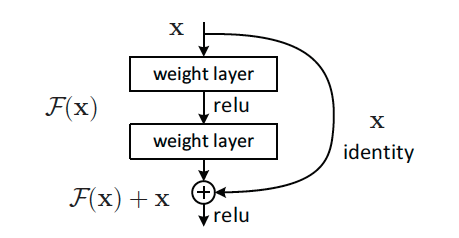
\includegraphics[width=0.5\textwidth]{images/residual_unit.png}
    \caption[The residual unit from ResNet]
          {A residual unit. The identity mapping is always present, and the
            network learns the difference from the identity mapping, $\mathcal{F}(x)$.
            Taken from \citep{he_deep_2015}.}
      \label{fig:residual_unit}
  \end{figure}

\section{Visualization Schemes}\label{sec:visualization_schemes}
  Since CNNs have become so good at a variety of tasks, it is more important
  now than ever to gain more insight into \emph{how} and \emph{what} they are
  learning. As described in the motivation for the project
  (\autoref{sec:motivation}), back projecting from the result to the input space
  can help improve a network's interpretability, and can even help improve its
  ability to learn. 

  \citeauthor{zeiler_adaptive_2011} first attempted to use `deconvolution' to
  improve their learning \citep{zeiler_adaptive_2011}, then later for purely
  visualization purposes \citep{zeiler_visualizing_compact_2014}. Their method
  involves mapping activations at different layers of the network back to the pixel
  space
  
  \autoref{fig:deconv_feature} shows the block diagram for how deconvolution is
  done. Inverting a convolutional layer is done by taking the 2D transpose of each
  slice of the filter. Inverting a ReLU is done by simply applying a ReLU again
  (ensuring only positive values can flow back through the network). Inverting
  a max pooling step is a little trickier, as max pooling is quite a lossy
  operation. \citeauthor{zeiler_adaptive_2011} get around this by saving extra
  information on the forward pass of the model --- switches that store the
  location of the input that caused the maximum value. This way, on the
  backwards pass, it is trivial to store activations to the right position in
  the larger feature map. Note that the positions that did not contribute to
  the max pooling operation remain as zero on the backwards pass. This is shown
  in \autoref{fig:deconv_switches}.

  \begin{figure}
    \centering
      % \includegraphics[width=0.9\textwidth]{images/deconv_block.png}
      \caption[Deconvolution Network Block Diagram]
              {A block diagram view of the model. Note the switches that
              are saved before the pooled features, and the filters
              used for deconvolution are the transpose of the filters used for
              a forward pass. Taken from
              \citep{zeiler_visualizing_compact_2014}.}
      \label{fig:deconv_feature}
  \end{figure}

  \begin{figure}
    \centering
      % \includegraphics[width=\textwidth]{images/deconv_switches.png}
      \caption[Unpooling operation in a deconvnet]
              {Unpooling operation in a deconvnet. On the forward pass, the
              locations of the maximum values are stored (the centre map with
              grey squares). This is then used on the backwards pass to put
              values at the correct location. Figure taken from \citep{zeiler_visualizing_compact_2014}.}
      \label{fig:deconv_switches}
  \end{figure}
  
  \autoref{fig:deconv_slices} gives a more detailed view of how the
  deconvolution works for convolutional layers.
  \begin{figure}
    \centering
      % \includegraphics[width=\textwidth]{images/deconv_layers.png}
      \caption[Deconvolution by slices]
              {Deconvolution by slices. 
              Visualization of 2 layers of the model showing how to invert
              a convolutional layer. At layer 2 of the model, there are $L$ feature
              maps $z_{l,2}$ (top green). Each of these feature
              maps was made from a different filter. The $L$ different filters
              are shown below the activations in red --- $f^c_{l,2}$. The
              $c$ superscript on these filters indexes the channel. E.g.\
              a convolutional filter could be $5\x 5\x 64$, where the first two
              indices the spatial support of the filter, and the third index
              --- the 64 --- is the fully connected depth aspect of the filter,
              the $c$ in this case. Each filter is laid out slice by slice. For
              simplicity, only two slices are shown in the figure. The
              2D transpose of this filter is taken and convolved with the
              feature map $z_{l,2}$. The result of this is $L\x C$ images. For
              each $c \in \{0\ldots C-1\}$, the $c$'th output from all $L$
              feature maps are summed together to make a pooled map $p_{c,1}$.
              These $C$ pooled maps are then expanded to make the $C$ feature
              maps at the layer below (indexed by k in the figure) --- $z_{k,2}$. 
              This process then repeats
              until we return to the input space. Not shown on this diagram are
              non-linear layers, but these are simple, point-wise operations.
              It would be trivial to insert them conceptually, by putting one
              more step, going from an intermediate feature map $z'_{k,1}$ to
              $z_{k,1}$. This figure was taken from
              \citep{zeiler_adaptive_2011}.}
      \label{fig:deconv_slices}
  \end{figure}

  \begin{figure}
    \centering
      % \makebox[\textwidth][c]{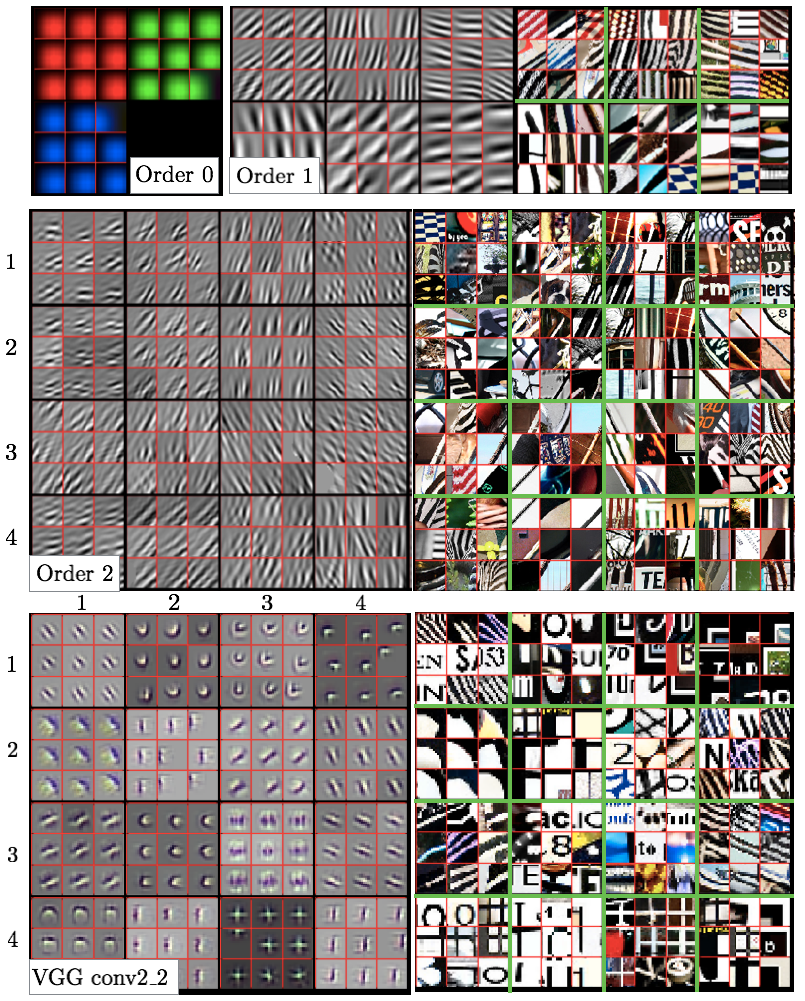
\includegraphics[width=1.1\textwidth]{images/deconv_images.png}}
      \caption[Visualization of deconvolved features]
              {Visualization of some deconvolved features.  9 coordinates are chosen in the
              feature map for layer 1 $z^1$, 16 for the second layer
              feature map $z^2$ and 16 for the third layer feature map.
              The entire dataset is run, and 9 images that made the largest
              activation at this point are noted. Deconvolution is then done on
              the feature maps from these 9 images, and the results are shown
              next to the actual images. Deeper layers are picking up more
              complex structures. Taken from \citep{zeiler_visualizing_compact_2014}.}
  \end{figure}

  \citeauthor{mahendran_understanding_2015} take a slightly different route on
  deconvolution networks \citep{mahendran_understanding_2015}. They do not
  store this extra information but instead define a cost function to maximize
  to. This results in visualization images that look very surreal, and can be
  quite different from the input.



